\chapter{Kravspecifikation (Alle)}

\section{Version}
\begin{table}[h]
	\centering
	\begin{tabularx}{\textwidth - 2cm}{|l|l|l|X|}
	\hline
	Dato	& Version	& Initialer & Ændring	\\ \hline
	26. februar & 1 & MHG & Første udkast. \\ \hline
	6. marts & 2 & MHG & Rettelser efter review. \\ \hline
	12. marts & 3 & MHG & Mindre rettelser efter fælles gennemlæsning. \\\hline
	\end{tabularx}
\end{table}

\section{Systembeskrivelse}
Under udviklingen af prototypen for AutoGreen, anvendes en drivhusmodel, der er vist på Figur \ref{fig:dimensioner}.

\begin{figure}[!h]
\centering 
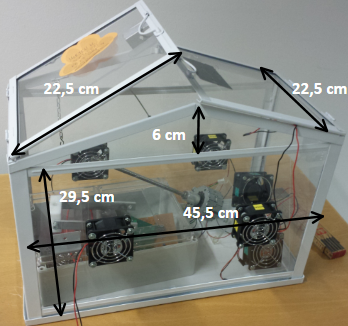
\includegraphics[scale=0.9] {../fig/dimensioner.png}
\caption{Dimensioner for drivhus.}
\label{fig:dimensioner}
\end{figure}

På billedet ses blæsere samt vinduesmotoren (ikke monteret). Disse indgår som en del af systemet, men selve drivhuset gør ikke. Der vil i systemet ydermere være et varmelegeme, som ikke er repræsenteret på billedet. 

\begin{figure}[!h]
\centering 
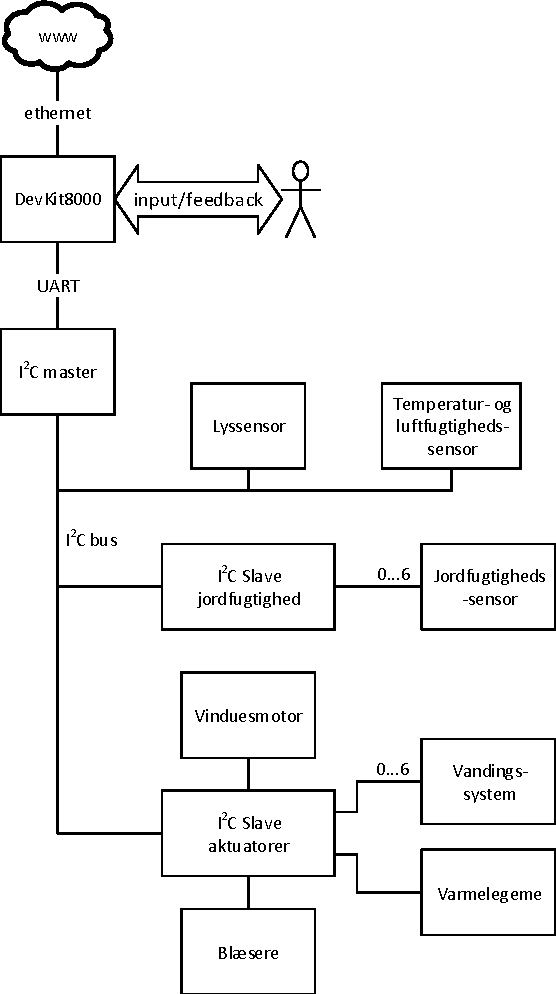
\includegraphics[height={\textheight - 2 cm}, trim=0 0 0 0, clip=true] {../fig/systemoversigt/sys_fig.pdf}
\caption{Oversigt over system}
\label{fig:systemoversigt}
\end{figure}

\clearpage

\subsubsection{DevKit8000}
DevKit8000 er systemets kontrolenhed og brugergrænseflade. 
DevKit8000 modtager input fra brugeren på dens touch skærm, og den kan give output til brugeren på skærmen og via e-mail; den er koblet til internet via ethernet. 
DevKit8000 kommunikerer vha. UART med en \IIC Master.
\subsubsection{\IIC Master}
I\textsuperscript{2}C Master er realiseret på et PSoC4 udviklingsboard (CY8CKIT-042). 
\IIC Master modtager input fra DevKit8000 og sender/modtager data til/fra \IIC Slaver, hvorefter respons sendes retur til DevKit8000.
\subsubsection{\IIC Slave Jordfugtighed}
\IIC Slave Jordfugtighed er ansvarlig for alle handlinger og målinger, der har at gøre med vanding i det fysiske drivhus. Der kan tilkobles 0 - 6 jordfugtighedssensorer med tilhørende aktuator til et evt. vandingssystem. Selve vandingssystemet er ikke en del af AutoGreen, en vandingsaktuator er en high/low bool. Enheden er realiseret på et PSoC4 udviklingsboard (CY8CKIT-042).
\subsubsection{\IIC Slave Aktuatorer}
\IIC Slave Aktuatorer er ansvarlig for al kommunikation mellem \IIC Master og alle aktuatorer i det fysiske drivhus. Enheden er realiseret på et PSoC4 udviklingsboard (CY8CKIT-042).

\section{Ordforklaring}

\subsubsection{Plantedatabase}
Plantedatabasen indeholder information om ideelle forhold for forskellige typer planter, som brugeren kunne tænkes at plante i sit fysiske drivhus. 
Informationen i plantedatabasen står til grund for udgangsparametre for nye planter i det virtuelle drivhus. Der findes en række systemplanter, som brugeren ikke kan redigere eller slette, men brugeren kan tilføje egne planter.
\subsubsection{Data Log}
Systemet er udstyret med en log over de indsamlede data fra sensorer i systemet, der måles og indskrives i loggen hvert minut. 
Denne er opbygget som en database, hvor hver logning indeholder information fra de diskrete sensorer samt et tidspunkt. 
\subsubsection{System Log}
Systemet er udstyret med en log over hvad systemet foretager sig. 
Dette kunne f.eks. være et indlæg når systemet foretager en måling, sender en e-mail, regulerer miljøet i drivhuset.
\subsubsection{Virtuelt Drivhus}
Det virtuelle drivhus er systemets repræsentation af det fysiske drivhus. Brugeren kan tilføje planter fra plantedatabasen i det virtuelle drivhus, og på den måde give systemet indirekte oplysninger om ønskede parametre.
Disse informationer lagres i systemets konfigurationsfil.
\subsubsection{Fysisk Drivhus}
Ved det fysiske drivhus forstås det drivhus hvori systemet er monteret. 
\subsubsection{Konfigurationsfil}
Dette er en automatisk genereret fil, der er placeret på DevKit8000, som indeholder brugerens konfigurationer om blandt andet notifikationer, e-mailadresser, antallet af fugtsensorer og deres unikke id mm.
\subsubsection{Notifikations E-mail}
Dette er en daglig E-mail, som brugeren kan vælge at få tilsendt. Den sendes klokken 12:00, og indeholder informationer om parametrene i det fysiske drivhus.
\subsubsection{Advarsels E-mail}
Dette er en E-mail, som brugeren kan vælge at få tilsendt. Den sendes, hvis en parameter i det fysiske drivhus kommer uden for tolerancen af den ønskede værdi.

\section{Brugerfladen}
\begin{figure}[h]
\centering
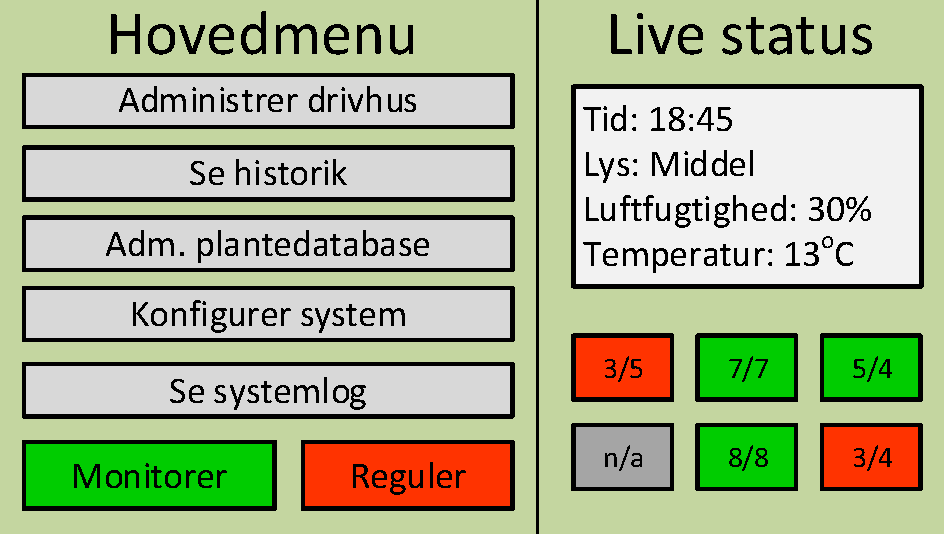
\includegraphics[width=\textwidth - 3 cm]{../fig/gui_skitse}
\caption{Skitse af hovedmenuen på brugerfladen.}
\label{fig:gui_skitse}
\end{figure}

I Figur \ref{fig:gui_skitse} er vist en skitse over hvordan brugerfladen forventes at se ud. De grå områder under Hovedmenu er knapper, brugeren kan trykke på for at tilgå yderligere menuer. 

Nederst ses "Monitorér" og "Regulér" knapper, som kan aktivere eller deaktivere hhv. monitorerings- og reguleringsfunktionalitet. 

Til højre ses live status for det fysiske drivhus. Nederst ses live status for jordfugtighed for hver plante. Dette er vist ved seks felter i forskellige farver. Disse symboliserer planter i det virtuelle drivhus, og viser status for den enkelte plante. Grøn betyder at plantens jordfugtighed er indenfor tolerancerne, hvor rød betyder at den er uden for tolerancen. Grå (Not Available) betyder, at der ikke er placeret en plante i det virtuelle drivhus, for den pågældende fugtighedssensor. 

\section{Aktør Kontekst Diagram} 
\begin{figure}[h]
\centering 
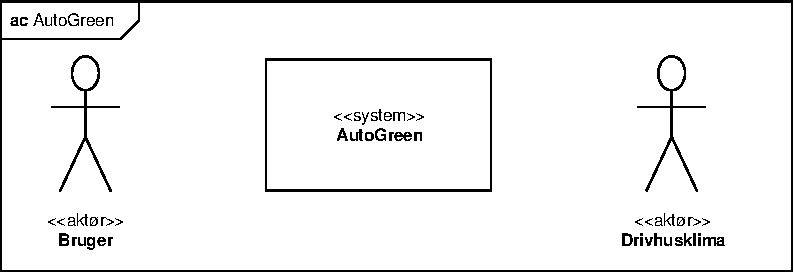
\includegraphics[width={\textwidth}, trim=0 0 0 0, clip=true] {../fig/Aktoer_Kontekst_Diagram.pdf}
\caption{Aktør Kontekst Diagram for AutoGreen}
\label{fig:aktoer_kontekst_diagram}
\end{figure}

\subsection{Aktørbeskrivelser}

\subsubsection{Bruger - Primær Aktør}
Brugeren kan:
\begin{itemize}
\item Starte og stoppe systemet 
\item Overvåge det aktuelle klima i drivhuset. 
\item Administrere drivhuset, hvilket vil sige at han giver systemet input om hvilke planter der er i drivhuset. 
\item Se historik over klimaet i drivhuset
\item Konfigurere systemindstillinger
\item Se systemlog
\item Modtage rapportering om klimaet i drivhuset 
\item Administrere planter i plantedatabasen
\end{itemize}

\subsubsection{Drivhusklima - Sekundær Aktør}
Drivhusklimaet består af en række parametre, som systemet måler og/eller regulerer:
\begin{itemize}
\item Lufttemperatur
	\subitem Måles, registreres og reguleres af systemet. Reguleringen sker vha. vinduesåbner, blæsere og varmelegeme.
\item Jordfugtighed
	\subitem Måles, registreres og reguleres indirekte af systemet
\item Luftfugtighed
	\subitem Måles og registreres af systemet
\item Lysintensitet
	\subitem Måles og registreres af systemet
\end{itemize}

\section{Funktionelle Krav}
Systemet\ldots
\begin{enumerate}\itemsep1pt \parskip0pt \parsep0pt
	\item \ldots \emph{Skal} give brugeren mulighed for at monitorere og konfigurere drivhusklimaet vha. en grafisk brugerflade på et touch display.
	\item \ldots \emph{Skal} have mulighed for at starte og stoppe systemet.
	\item \ldots \emph{Skal} måle lufttemperatur i det fysiske drivhus.
	\item \ldots \emph{Skal} kunne regulere temperatur i det fysiske drivhus.
	\item \ldots \emph{Skal} kunne indstilles til brugerdefineret tid og dato.
	\item \ldots \emph{Skal} kunne give brugeren mulighed for at vælge brug af varmelegeme og ventilatorer.
	\item \ldots \emph{Skal} give brugeren mulighed for at tilføje en plante i det virtuelle drivhus.
	\item \ldots \emph{Skal} give brugeren mulighed for at fjerne en plante i det virtuelle drivhus.
	\item \ldots \emph{Skal} give brugeren mulighed for at redigere en plante i det virtuelle drivhus.
	\item \ldots \emph{Skal} kunne regulere drivhusklima automatisk efter behov.
	\item \ldots \emph{Bør} kunne måle jordfugtighed i fysiske drivhus.
	\item \ldots \emph{Bør} kunne måle lysintensitet i det fysiske drivhus.
	\item \ldots \emph{Bør} kunne måle luftfugtighed i det fysiske drivhus.
	\item \ldots \emph{Bør} indeholde informationer om planter i en datastruktur.
	\item \ldots \emph{Bør} kunne fremvise grafisk historik over måledata fra drivhus.
	\item \ldots \emph{Bør} kunne vise planteinformationer fra plantedatabasen.
	\item \ldots \emph{Bør} give brugeren mulighed for at se en systemlog over hændelser i systemet.
	\item \ldots \emph{Bør} gemme alt monitorering i en data log.
	\item \ldots \emph{Kan} give brugeren mulighed for at redigere og slette planter i plantedatabasen, som brugeren selv har tilføjet.
	\item \ldots \emph{Kan} give brugeren mulighed for at tilføje/redigere/slette e-mail adresser.
	\item \ldots \emph{Kan} give brugeren mulighed for valg af varslings e-mail omhandlende dårligt klima og daglig e-mail.
	\item \ldots \emph{Kan} sende e-mail til brugeren, på baggrund af brugerindstillinger.
\end{enumerate}

\section{Ikke Funktionelle Krav}
Systemet\ldots
\begin{enumerate}\itemsep1pt \parskip0pt \parsep0pt
	\item \ldots \emph{Skal} minimum måle parametre i det fysiske drivhus med 1 minuts mellemrum +/- 5 sekunder.
	\item \ldots \emph{Skal} kunne justere temperaturen i det fysiske drivhus til det ønskede niveau på højst 30 minutter ved en starttemperatur der ligger højst 10 grader fra det ønskede niveau, når alle tre aktuatorer anvendes.
	\item \ldots \emph{Skal} kunne måle jordfugtighed i trin á 10, hvor 10 er mest fugtigt. 
	\item \ldots \emph{Skal} kunne indeholde op til seks fugtmålere.
	\item \ldots \emph{Skal} kunne indeholde op til 100 planter i plantedatabasen.
	\item \ldots \emph{Skal} kunne indeholde måledata et år tilbage i tiden.
	\item \ldots \emph{Skal} kunne måle temperaturen med en præcision på +/- 1 grad celcius ved 20 grader.
	\item \ldots \emph{Skal} kunne indeholde op til tre e-mail adresser.
	\item \ldots \emph{Bør} kunne justere temperaturen til 25 grader celcius i det fysiske drivhus med en præcision på +/- 2 grad, når drivhuset er placeret i et rum ved stuetemperatur (ca. 20 grader).
	\item \ldots \emph{Kan} sende mail til brugeren højest 1 minut efter et for lavt jordfugtighedsniveau er målt, hvis den er indstillet til dette.
\end{enumerate}


\section{Use Case Diagram}
\begin{figure}[h]
\centering 
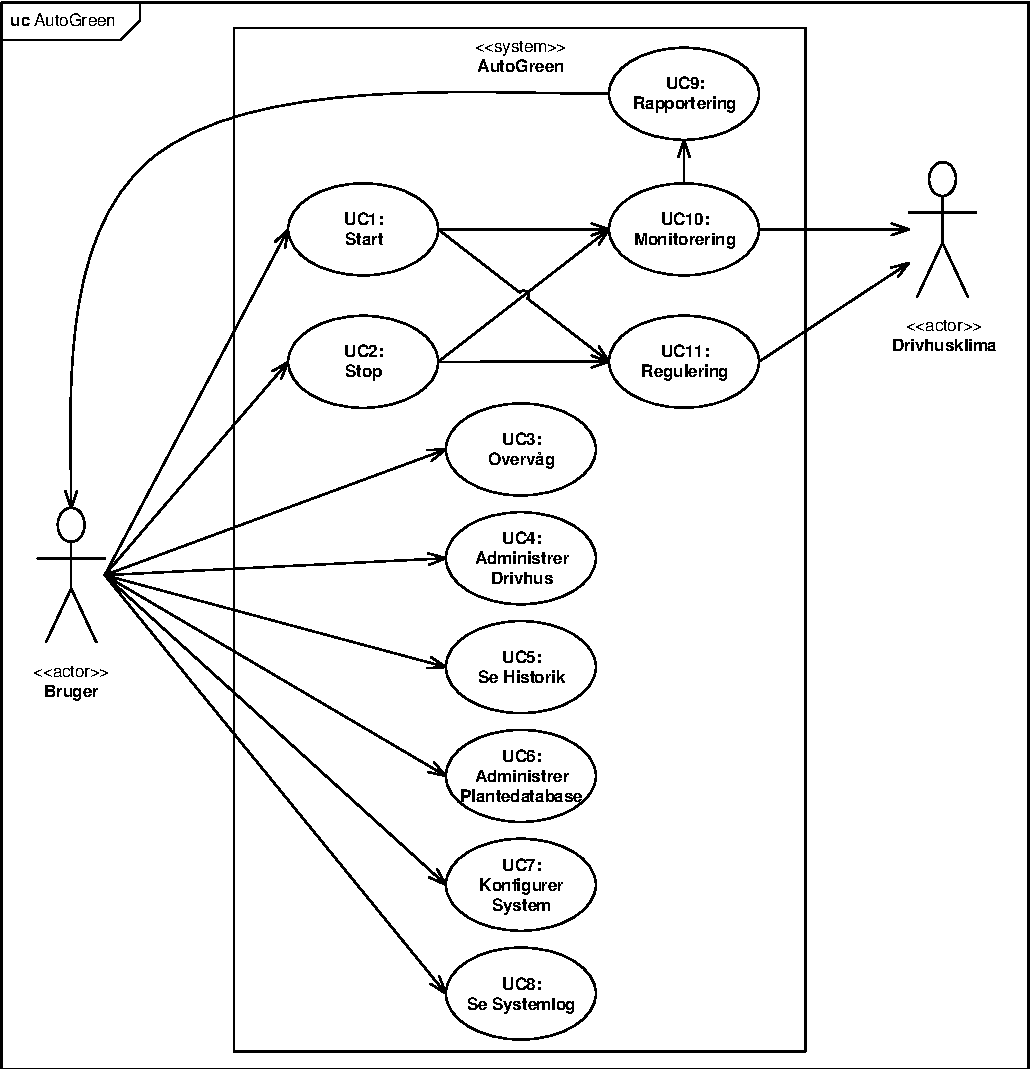
\includegraphics[width={\textwidth-1cm}, trim=0 0 0 0, clip=true] {../fig/UC_Diagram.pdf}
\caption{Use Case Diagram for AutoGreen}
\label{fig:use_case_diagram}
\end{figure}

\clearpage

\subsection{Use Case beskrivelser - Initiering og Formål}
\subsubsection{UC1: Start}
Initieres af: Bruger

Denne UC giver brugeren mulighed for at starte systemet, dvs. monitorering og regulering af drivhusklimaet. 
Brugeren har mulighed for kun at starte monitorering. Use Case’en kan initiere UC10 Rapportering og UC11 Monitorering.

\subsubsection{UC2: Stop}
Initieres af: Bruger

Denne UC giver brugeren mulighed for at stoppe systemet, dvs. monitorering og regulering af drivhusklimaet. 
Brugeren har mulighed for kun at stoppe regulering. Use Case’en kan stoppe UC10 Rapportering og UC11 Monitorering.

\subsubsection{UC3: Overvåg}
Initieres af: Bruger

Når UC10 Monitorering er startet, vises der i user interfacets hovedmenu live opdaterede måleværdier. 
Såfremt UC11 Regulering er startet, kan værdierne for lufttemperatur og jordfugtighed være røde, hvis de ikke passer med de ønskede værdier.

\subsubsection{UC4: Administrer Drivhus}
Initieres af: Bruger

Denne UC giver brugeren mulighed for at informere systemet om hvilke planter der er i drivhuset. 
Brugeren kan tilføje op til seks planter fra plantedatabasen i det virtuelle drivhus, og brugeren kan redigere parametre for disse, hvis brugeren ønsker andre parametre end dem, der fremgår i plantedatabasen. 
Hver af disse planter kan forbindes med en jordfugtighedsmåler. 

\subsubsection{UC5: Se Historik}
Initieres af: Bruger

Denne Use Case giver brugeren mulighed for at se grafisk historik over de fire målte parametre i drivhuset. 
Brugeren kan se data op til et år tilbage i tiden. 

\subsubsection{UC6: Administrer Plantedatabase}
Initieres af: Bruger

Denne UC giver brugeren mulighed for at se på planter i databasen. 
Brugeren kan desuden tilføje og fjerne egne planter i databasen, og brugeren kan redigere i de planter brugeren tidligere har tilføjet. 

\subsubsection{UC7: Konfigurer System}
Initieres af: Bruger

Denne UC giver brugeren mulighed for at rette i systemindstillinger, herunder:
\begin{packed_item}
\item Indstille tid og dato
\item Tilføje/fjerne/rette e-mail adresse 
\item Aktivering/deaktivering af advarsels E-mail
\item Aktivering/deaktivering af notifikations E-mail
\item Aktivering/deaktivering af varmelegeme
\item Aktivering/deaktivering af luftcirkulation
\end{packed_item}

\subsubsection{UC8: Se System Log}
Initieres af: Bruger

Denne UC giver brugeren mulighed for at se en liste over systemhændelser, herunder:
\begin{packed_item}
\item Start og stop af system
\item Manglende kontakt til sensorer
\item Afsendte e-mails
\item Tilføjede/fjernede/redigerede planter i drivhuset
\item Tilføjede/fjernede/redigerede planter i plantedatabasen
\item Konfigurationsændringer
\item Fejl i registrering i data log
\item Fejl på vinduesåbner
\item Fejl på luftcirkulation
\item Fejl på varmelegeme
\item Foretaget regulering
\end{packed_item}

\subsubsection{UC9: Rapportering}
Initieres af: UC10 Monitorering

Denne Use Case rapporterer til brugeren ud fra de indstillinger brugeren har valgt under UC7 Konfigurer System. 
Dette sker ved afsendelse af e-mail til den eller de adresser, som brugeren ligeledes har tilføjet under UC7 Konfigurer System.

\subsubsection{UC10: Monitorering}
Initieres af: UC1 Start.

Denne Use Case lagrer målinger af lufttemperatur, jordfugtighed, luftfugtighed og lysintensitet i en data log fil. 
Lagringen sker minimum en gang i minuttet. 

\subsubsection{UC11: Regulering}
Initeres af: UC1 Start.

Denne Use Case regulerer temperaturen i drivhuset, vha. vinduesåbner, varmelegeme og luftcirkulation, med mindre brugeren har slået varmelegeme og/eller luftcirkulation fra. 
Det kan ske uden luftcirkulation og/eller varmelegeme, hvis brugeren har valgt dette under UC7 Konfigurer System. Det er ikke muligt at aktivere regulering uden at UC10 Monitorering er aktiveret.

\clearpage

\subsection{Use Case Beskrivelser - Fully Dressed}
For alle Use Cases hvor brugeren navigerer i undermenuer af hovedmenuen, gælder det, at brugeren har mulighed for at gå et skridt tilbage ved at trykke på en ”tilbage knap”. Fremover ved benævningen ”Systemet er operationelt” menes, at systemet er tilsluttet strømforsyning og at alt fungerer samt at systemet er tilsluttet ethernet.

%UC1
\begin{table}[h]
\begin{tabularx}{\textwidth}{| >{\raggedright\arraybackslash}p{3.3 cm} | >{\raggedright\arraybackslash}X |} \hline

\textbf{Navn:} 						& UC1: Start\\ \hline
\textbf{Mål:}						& At starte systemet helt eller delvist. \\ \hline
\textbf{Initering:}					& Bruger \\ \hline
\textbf{Aktører:} 					& Bruger (primær) \\ \hline
\textbf{Reference:} 					& UC10: Monitorering, UC11: Regulering \\ \hline
\textbf{Antal samtidige forekomster:} & Én \\ \hline
\textbf{Forudsætning:} 				& Systemet er stoppet helt, er operationelt og viser hovedmenuen.\\ \hline
\textbf{Resultat:}					& UC10: Monitorering og evt. UC11: Regulering er startet, systemet viser Hovedmenuen. \\ \hline
\textbf{Hovedscenarie:}				& 

\begin{packed_enum}
\item Bruger trykker på "Monitorering". 
\item System aktiverer UC10: Monitorering. 
\item Bruger trykker på "Regulering". 
	\begin{packed_item}\itemsep1pt \parskip0pt \parsep0pt
	\item {[}Ext 3.a : Bruger trykker ikke "Regulering".{]}
	\end{packed_item}
\item Systemet aktiverer UC11: Regulering.
\item UC1 afsluttes.
\end{packed_enum} \\ \hline
\textbf{Udvidelser:}				&  
\textbf{{[}Ext 3.a : Bruger vælger kun monitorering.{]}}
	\begin{packed_enum}\itemsep1pt \parskip0pt \parsep0pt
	\item Systemet fortsætter ved pkt. 5 i hovedscenariet.
	\end{packed_enum}
\\ \hline
\end{tabularx}
\caption{UC1: Start}
\label{tbl:UC1}
\end{table}

\clearpage
%UC2
\begin{table}[h]
\begin{tabularx}{\textwidth}{| >{\raggedright\arraybackslash}p{3.3 cm} | >{\raggedright\arraybackslash}X |} \hline

\textbf{Navn:} 						& UC2: Stop\\ \hline
\textbf{Mål:}						& At stoppe systemet helt eller delvist. \\ \hline
\textbf{Initering:}					& Bruger \\ \hline
\textbf{Aktører:} 					& Bruger (primær) \\ \hline
\textbf{Reference:} 					& UC10: Monitorering, UC11: Regulering \\ \hline
\textbf{Antal samtidige forekomster:} & Én \\ \hline
\textbf{Forudsætning:} 				& Både UC10: Monitorering og UC11: Regulering er startet, systemet er operationelt og viser hovedmenuen.\\ \hline
\textbf{Resultat:}					& UC10: Monitorering og evt. UC11: Regulering er stoppet, systemet viser Hovedmenuen. \\ \hline
\textbf{Hovedscenarie:}				& 

\begin{packed_enum}
\item Bruger trykker på monitorerings knap. 
	\begin{packed_item} \itemsep1pt \parskip0pt \parsep0pt
		\item {[} Ext 1.a: Bruger trykker på regulerings knap.{]}
	\end{packed_item}
\item System stopper UC10: Monitorering og UC11: Regulering.
\item UC2 afsluttes.

\end{packed_enum} \\ \hline
\textbf{Udvidelser:}				&  
\textbf{{[}Ext 1.a : Bruger trykker på regulerings knap.{]}}
	\begin{packed_enum}\itemsep1pt \parskip0pt \parsep0pt
	\item Systemet stopper UC11: Regulering.
	\item Systemet fortsætter ved pkt. 3 i hovedscenariet.
	\end{packed_enum}
\\ \hline
\end{tabularx}
\caption{UC2: Stop}
\label{tbl:UC2}
\end{table}

\begin{table}[h]
\begin{tabularx}{\textwidth}{| >{\raggedright\arraybackslash}p{3.3 cm} | >{\raggedright\arraybackslash}X |} \hline

\textbf{Navn:} 						& UC3: Overvåg\\ \hline
\textbf{Mål:}						& At se aktuel status i det fysiske drivhus i Hovedmenuen. \\ \hline
\textbf{Initering:}					& Bruger \\ \hline
\textbf{Aktører:} 					& Bruger (primær) \\ \hline
\textbf{Reference:} 					& Ingen \\ \hline
\textbf{Antal samtidige forekomster:} & Én \\ \hline
\textbf{Forudsætning:} 				& UC10: Monitorering er aktiv, systemet er operationelt og hovedmenuen vises. \\ \hline
\textbf{Resultat:}					& Brugeren har set et live feed af parametre for det fysiske drivhus. \\ \hline
\textbf{Hovedscenarie:}				& ~

\begin{packed_enum}
\item Bruger aflæser måleværdier på brugerfladen.
\item UC3 afsluttes.
\end{packed_enum} \\ \hline
\textbf{Udvidelser:}				& ~
Ingen \\ \hline
\end{tabularx}

\clearpage

\caption{UC3: Overvåg}
\label{tbl:UC3}
\end{table}

\begin{table}[h]
\begin{tabularx}{\textwidth}{| >{\raggedright\arraybackslash}p{3.3 cm} | >{\raggedright\arraybackslash}X |} \hline

\textbf{Navn:} 						& UC4: Administrer Drivhus\\ \hline
\textbf{Mål:}						& Bruger har informeret systemet om hvilke planter, der er i drivhuset. \\ \hline
\textbf{Initering:}					& Bruger \\ \hline
\textbf{Aktører:} 					& Bruger (primær) \\ \hline
\textbf{Reference:} 					& Ingen \\ \hline
\textbf{Antal samtidige forekomster:} & Én \\ \hline
\textbf{Forudsætning:} 				& Systemet er operationelt og hovedmenuen vises.\\ \hline
\textbf{Resultat:}					& Konfigureringsfilen er opdateret med informationer fra brugeren. \\ \hline
\textbf{Hovedscenarie:}				& 

\begin{packed_enum}
\item Bruger trykker på ”Administrer drivhus” i hovedmenu.
\item System viser "Virtuel Drivhus Menu". 
\item Bruger trykker på ”Tilføj plante”.
	\begin{packed_item}\itemsep1pt \parskip0pt \parsep0pt
	\item {[}Alt 3.a : Bruger trykker på en plante, der skal fjernes.{]}
	\end{packed_item}
	\begin{packed_item}\itemsep1pt \parskip0pt \parsep0pt
	\item {[}Alt 3.b : Bruger trykker på en plante, der skal redigeres.{]}
	\end{packed_item}
\item System præsenterer bruger for liste af planter i Plantedatabasen.
\item Bruger trykker på den plante, der skal tilføjes.
\item Systemet opretter planten i det virtuelle drivhus med parametrene fra plantedatabasen.
\item System viser "Planteredigeringsmenu".
\item Bruger redigerer ønskede parametre og trykker "OK".
\item Systemet gemmer brugerens valg i konfigurationsfilen og præsenterer "Virtuel Drivhus Menu".
\item Bruger trykker "Tilbage".
\item UC4 afsluttes og systemet viser Hovedmenu.
\end{packed_enum} \\ \hline

\textbf{Alternativ:}				& 
\textbf{{[}Alt 3.a : Bruger trykker på en plante, der skal fjernes.{]}}
\begin{packed_enum}
\setcounter{enumi}{3}
\item System viser "Planteredigeringsmenu".
\item Bruger trykker på ”Fjern”.
\item Systemet fjerner planten fra det virtuelle drivhus og markerer planten som fjernet i data loggen.
\item Systemet præsenterer "Virtuel Drivhus Menu".
\item UC4 fortsætter fra pkt. 10 i hovedscenariet.
\end{packed_enum}
\textbf{{[}Alt 3.b : Bruger trykker på en plante, der skal redigeres.{]}}
\begin{packed_enum}
\setcounter{enumi}{3}
\item UC4 fortsætter fra pkt. 7 i hovedscenariet.
\end{packed_enum}
\\ \hline

\textbf{Udvidelser:}				&  
Ingen
\\ \hline
\end{tabularx}
\caption{UC4: Administrer Drivhus}
\label{tbl:UC4}
\end{table}

\clearpage

\begin{table}[h]
\begin{tabularx}{\textwidth}{| >{\raggedright\arraybackslash}p{3.3 cm} | >{\raggedright\arraybackslash}X |} \hline

\textbf{Navn:} 						& UC5: Se Historik\\ \hline
\textbf{Mål:}						& At se historik fra data loggen op til et år tilbage. \\ \hline
\textbf{Initering:}					& Bruger \\ \hline
\textbf{Aktører:} 					& Bruger (primær) \\ \hline
\textbf{Reference:} 					& Ingen \\ \hline
\textbf{Antal samtidige forekomster:} & Én \\ \hline
\textbf{Forudsætning:} 				& Systemet er operationelt og hovedmenuen vises. \\ \hline
\textbf{Resultat:}					& Brugeren har set historik, systemet viser Hovedmenuen. \\ \hline
\textbf{Hovedscenarie:}				& 

\begin{packed_enum}
\item Bruger trykker ”Se Historik” i hovedmenu.
\item System viser "Historikmenu". 
\item Bruger vælger den ønskede tidshorisont (uge/måned/år).
\item Systemet viser en graf over den valgte periode.
\item Bruger kan nu vælge at deaktivere nogle måleværdier. Lys, temperatur, luftfugtighed kan deaktiveres således at de kan vises hver for sig eller samtidigt. Desuden kan brugeren vælge mellem jordfugtighed for planter i drivhuset.
\item Bruger trykker "Tilbage", UC5 afsluttes og Hovedmenuen vises.
\end{packed_enum} \\ \hline
\end{tabularx}
\caption{UC5: Se Historik}
\label{tbl:UC5}
\end{table}

\clearpage

\begin{table}[h]
\begin{tabularx}{\textwidth}{| >{\raggedright\arraybackslash}p{3.3 cm} | >{\raggedright\arraybackslash}X |} \hline

\textbf{Navn:} 						& UC6: Administrer Plantedatabase\\ \hline
\textbf{Mål:}						& At administrere planter i plantedatabasen. \\ \hline
\textbf{Initering:}					& Bruger \\ \hline
\textbf{Aktører:} 					& Bruger (primær) \\ \hline
\textbf{Reference:} 					& Ingen \\ \hline
\textbf{Antal samtidige forekomster:} & Én \\ \hline
\textbf{Forudsætning:} 				& Systemet er operationelt og hovedmenuen vises. \\ \hline
\textbf{Resultat:}					& Brugeren har tilføjet, redigeret og/eller fjernet plante i plantedatabasen. Systemet viser Hovedmenuen.\\ \hline
\textbf{Hovedscenarie:}				& 

\begin{packed_enum}
\item Bruger trykker ”Administrer Plantedatabase” i hovedmenu.
\item System viser "Plantedatabasemenu". 
\item Bruger trykker på "Tilføj Data". 
	\begin{packed_item}\itemsep1pt \parskip0pt \parsep0pt
	\item {[}Alt 3.a : Bruger trykker på en plante, der skal fjernes. {]}
	\end{packed_item}
	\begin{packed_item}\itemsep1pt \parskip0pt \parsep0pt
	\item {[}Alt 3.b : Bruger trykker på en plante, der skal redigeres. {]}
	\end{packed_item}
\item Systemet opretter en plante med standardparametre og præsenterer "Databaseredigeringsmenu".
\item Bruger redigerer ønskede parametre og trykker "OK".
\item Systemet gemmer brugerens valg og viser "Plantedatabasemenu".
\item Bruger trykker "Tilbage".
\item UC6 afsluttes og systemet viser Hovedmenuen.
\end{packed_enum} \\ \hline

\textbf{Alternativ:}				& 
\textbf{{[}Alt 3.a : Bruger trykker på en plante, der skal fjernes.{]}}
\begin{packed_enum}
\setcounter{enumi}{3}
\item System viser "Databaseredigeringsmenu".
\item Bruger vælger "Fjern Data" og trykker "OK".
\item Systemet fjerner planten fra Plantedatabasen og viser "Plantedatabasemenu".
\item UC6 fortsætter fra pkt. 7 i hovedscenariet. 
\end{packed_enum}
\textbf{{[}Alt 3.b : Bruger trykker på en plante, der skal redigeres.{]}}
\begin{packed_enum}
\setcounter{enumi}{3}
\item Systemet viser "Databaseredigeringsmenu".
\item UC6 fortsætter fra pkt. 5 i hovedscenariet.
\end{packed_enum}
\\ \hline

\textbf{Udvidelser:}				&  
Ingen
\\ \hline
\end{tabularx}
\caption{UC6: Administrer Plantedatabase}
\label{tbl:UC6}
\end{table}

\clearpage

\begin{table}[!h]
\begin{tabularx}{\textwidth}{| >{\raggedright\arraybackslash}p{3.3 cm} | >{\raggedright\arraybackslash}X |} \hline
\textbf{Navn:} 						& UC7: Konfigurer System\\ \hline
\textbf{Mål:}						& At konfigurere indstillinger for systemet. \\ \hline
\textbf{Initering:}					& Bruger \\ \hline
\textbf{Aktører:} 					& Bruger (primær) \\ \hline
\textbf{Reference:} 					& Ingen \\ \hline
\textbf{Antal samtidige forekomster:} & Én \\ \hline
\textbf{Forudsætning:} 				& Systemet er operationelt, regulering er aktiveret og hovedmenuen er vist. \\ \hline
\textbf{Resultat:}					& Systemet er konfigureret efter brugerens ønske. Hovedmenuen vises. \\ \hline
\textbf{Hovedscenarie:}				& 

\begin{packed_enum}
\item Bruger trykker ”Konfigurer System”.
\item System viser "Konfigurationsmenu". 
\item Bruger vælger "E-mail Adresser”. 
	\begin{packed_item}\itemsep1pt \parskip0pt \parsep0pt
	\item {[}Alt 3.a : Bruger vælger ”Notifikationer”.{]}
	\end{packed_item}
	\begin{packed_item}\itemsep1pt \parskip0pt \parsep0pt
	\item {[}Alt 3.b : Bruger vælger ”Indstil dato/tid”.{]}
	\end{packed_item}
	\begin{packed_item}\itemsep1pt \parskip0pt \parsep0pt
	\item {[}Alt 3.c : Bruger vælger ”Hardware indstillinger”.{]}
	\end{packed_item}
\item Systemet viser "E-mail menu".
\item Brugeren indtaster op til tre ønskede E-mail adresser og trykker "OK".
\item Systemet gemmer E-mail adresserne i konfigurationsfilen. Systemet viser "Konfigurationsmenu".
\item Brugeren trykker "tilbage".
\item UC7 afsluttes og Hovedmenuen vises.

\end{packed_enum} \\ \hline
\textbf{Alternativ:}				&  
\textbf{{[}Alt 3.a : Bruger vælger ”Notifikationer”.{]}}
	\begin{packed_enum}\itemsep1pt \parskip0pt \parsep0pt
	\setcounter{enumi}{3}
	\item System  viser "Notifikationsmenu".
	\item Brugeren indtaster ønskede indstillinger for notifikationer.
	\item Brugeren trykker "OK".
	\item Systemet gemmer indstillingerne i konfigurationsfilen og viser "Konfigurationsmenu".
	\item UC7 fortsætter fra punkt 7 i hovedscenariet.
	\end{packed_enum}
\textbf{{[}Alt 3.b : Bruger vælger ”Indstil dato/tid”.{]}}
	\begin{packed_enum}\itemsep1pt \parskip0pt \parsep0pt
	\setcounter{enumi}{3}
	\item Systemet viser "Tid- og datomenu".
	\item Bruger indtaster dato og tid.
	\item Brugeren trykker "OK".
	\item System gemmer de indtastede data i konfigurationsfilen og viser "Konfigurationsmenu".
	\item UC7 fortsætter fra punkt 7. 
	\end{packed_enum}
\textbf{{[}Alt 3.c : Bruger vælger ”Hardware indstillinger”.{]}}
	\begin{packed_enum}\itemsep1pt \parskip0pt \parsep0pt
	\setcounter{enumi}{3}
	\item System viser "Hardware Indstillingsmenu".
	\item Brugeren vælger blæser on/off og/eller varmelegeme on/off.
	\item Brugeren trykker "OK".
	\item System gemmer de indtastede indstillinger i konfigurationsfilen og viser "Konfigurationsmenu".
	\item UC7 fortsætter fra punkt 7 i hovedscenariet.
	\end{packed_enum}
\\ \hline
\end{tabularx}
\caption{UC7: Konfigurer System}
\label{tbl:UC7}
\end{table}

\clearpage

\begin{table}[h]
\begin{tabularx}{\textwidth}{| >{\raggedright\arraybackslash}p{3.3 cm} | >{\raggedright\arraybackslash}X |} \hline

\textbf{Navn:} 						& UC8: Se Systemlog\\ \hline
\textbf{Mål:}						& Brugeren aflæser data i system log. \\ \hline
\textbf{Initering:}					& Bruger \\ \hline
\textbf{Aktører:} 					& Bruger \\ \hline
\textbf{Reference:} 				& Ingen \\ \hline
\textbf{Antal samtidige forekomster:} & Én \\ \hline
\textbf{Forudsætning:} 				& Systemet er operationelt og hovedmenu vises. \\ \hline
\textbf{Resultat:}					& Brugeren har set system log og Hovedmenuen er vist. \\ \hline
\textbf{Hovedscenarie:}				& 

\begin{packed_enum}
\item Bruger vælger ”Se Systemlog”.
\item Systemet viser en "Systemlogmenu", der indeholder en liste over hændelser i systemet.
\item Bruger vælger ”Tilbage”.
\item UC8 afsluttes og hovedmenuen vises. 
\end{packed_enum} \\ \hline
\textbf{Udvidelser:}				&  
Ingen
\\ \hline
\end{tabularx}
\caption{UC8: Se Systemlog}
\label{tbl:UC8}
\end{table}

%UC9
\begin{table}[h]
\begin{tabularx}{\textwidth}{| >{\raggedright\arraybackslash}p{3.3 cm} | >{\raggedright\arraybackslash}X |} \hline

\textbf{Navn:} 						& UC9: Rapportering\\ \hline
\textbf{Mål:}						& Bruger modtager notifikations- og advarsels E-mails. \\ \hline
\textbf{Initering:}					& UC10: Monitorering \\ \hline
\textbf{Aktører:} 					& Bruger \\ \hline
\textbf{Reference:} 					& UC10: Monitorering \\ \hline
\textbf{Antal samtidige forekomster:} & Én \\ \hline
\textbf{Forudsætning:} 				& UC10 er aktiv, systemet er operationelt og notifikations- og advarselsemail er slået til. \\ \hline
\textbf{Resultat:}					& Systemet har sendt notifikations- og advarsels E-mail. \\ \hline
\textbf{Hovedscenarie:}				& 

\begin{packed_enum}
\item Systemet sender daglig notifikations E-mail klokken 12.
\item Systemet sender advarsels E-mail, hvis en parameter i det fysiske drivhus er under den ønskede værdi. 
\end{packed_enum}
\\ \hline
\textbf{Udvidelser:}				&  
Ingen \\ \hline
\end{tabularx}
\caption{UC9: Rapportering}
\label{tbl:UC9}
\end{table}

\clearpage
 
\begin{table}[h]
\begin{tabularx}{\textwidth}{| >{\raggedright\arraybackslash}p{3.3 cm} | >{\raggedright\arraybackslash}X |} \hline

\textbf{Navn:} 						& UC10: Monitorering\\ \hline
\textbf{Mål:}						& At opdatere live parametre i Hovedmenuen. \\ \hline
\textbf{Initering:}					& UC1: Start \\ \hline
\textbf{Aktører:} 					& Drivhusklima \\ \hline
\textbf{Reference:} 					& UC1: Start, UC2: Stop, UC9: Rapportering \\ \hline
\textbf{Antal samtidige forekomster:} & Én \\ \hline
\textbf{Forudsætning:} 				& UC1 er gennemført og systemet er operationelt. \\ \hline
\textbf{Resultat:}					& Hovedmenuen er opdateret med nyeste data fra data loggen. \\ \hline
\textbf{Hovedscenarie:}				& 

\begin{packed_enum}
\item Systemet indlæser konfigurationsfilen.
\item Systemet aflæser måleværdier fra sensorer og gemmer dem i data loggen. 
\item Systemet opdaterer live-status i hovedmenuen med de målte værdier.
\item Systemet sammenligner aflæste værdier fra sensorerne med ønskede værdier fra det virtuelle drivhus.
\item Målte værdier ligger inden for tolerancerne i forhold til ønskede værdier.
	\begin{packed_item}\itemsep1pt \parskip0pt \parsep0pt
	\item {[}Ext 4.a : Værdierne ligger ikke inden for tolerancerne.{]}
	\end{packed_item}
\item Systemet farver alle datafelter for jordfugtighed grønne.
\item Systemet venter et minut og fortsætter fra pkt. 1 i hovedscenariet.
\end{packed_enum} \\ \hline
\textbf{Udvidelser:}				&  
\textbf{{[}Ext 4.a : Værdierne ligger ikke inden for tolerancerne.{]}}
	\begin{packed_enum}\itemsep1pt \parskip0pt \parsep0pt
	\item Systemet aktiverer UC9: Rapportering.
	\item Systemet markerer datafelter, der ligger udenfor tolerancerne røde.
	\item Systemet fortsætter fra pkt. 7 i hovedscenariet.
	\end{packed_enum}
\\ \hline
\end{tabularx}
\caption{UC10: Monitorering}
\label{tbl:UC10}
\end{table}

\clearpage

%UC11
\begin{table}[h]
\begin{tabularx}{\textwidth}{| >{\raggedright\arraybackslash}p{3.3 cm} | >{\raggedright\arraybackslash}X |} \hline

\textbf{Navn:} 						& UC11: Regulering\\ \hline
\textbf{Mål:}						& At regulere temperaturen i det fysiske drivhus til ønsket værdi, samt at jordfugtigheden for hver plante stemmer overens med den angivne jordfugtighed i det virtuelle drivhus. \\ \hline
\textbf{Initering:}					& UC1: Start \\ \hline
\textbf{Aktører:} 					& Drivhusklima \\ \hline
\textbf{Reference:} 					& UC1: Start \\ \hline
\textbf{Antal samtidige forekomster:} & Én \\ \hline
\textbf{Forudsætning:} 				& Systemet er operationelt og regulering er aktiveret. \\ \hline
\textbf{Resultat:}					& Aktuatorer for vindue, blæsere, varmelegeme og vanding er evt. aktiveret. \\ \hline
\textbf{Hovedscenarie:}				& 

\begin{packed_enum}
\item Systemet indlæser konfigurationsfilen.
\item Systemet sammenligner nyeste værdier for jordfugtighed fra data loggen med ønskede værdier fra det virtuelle drivhus.
\item Jordfugtværdierne ligger inden for tolerancerne.
	\begin{packed_item}\itemsep1pt \parskip0pt \parsep0pt
	\item {[}Ext 3.a : En eller flere jordfugtværdier ligger under tolerancen.{]}
	\end{packed_item}
\item Systemet sammenligner nyeste værdi for temperatur fra data loggen med angiven værdi i det virtuelle drivhus.
\item Værdien ligger inden for tolerancen.
	\begin{packed_item}\itemsep1pt \parskip0pt \parsep0pt
	\item {[}Ext 5.a : Værdien for temperatur ligger over tolerancen.{]}
	\end{packed_item}
	\begin{packed_item}\itemsep1pt \parskip0pt \parsep0pt
	\item {[}Ext 5.b : Værdien for temperatur ligger under tolerancen.{]}
	\end{packed_item}
\item Systemet venter 1 minut og fortsætter fra pkt. 1 i hovedscenariet.
\end{packed_enum} \\ \hline
\textbf{Udvidelser:}				&  
\textbf{{[}Ext 3.a : En eller flere jordfugtværdier ligger under tolerancen.{]}}
	\begin{packed_enum}\itemsep1pt \parskip0pt \parsep0pt
	\item Systemet aktiverer aktuator for vanding for den eller de planter der er under tolerancen.
	\item Systemet fortsætter fra pkt. 4 i hovedscenariet.
	\end{packed_enum}
\textbf{{[}Ext 5.a : Værdien for temperatur ligger over tolerancen.{]}}
	\begin{packed_enum}\itemsep1pt \parskip0pt \parsep0pt
	\item Systemet regulerer temperaturen nedad jf. konfigurationsfilen.
	\item Systemet fortsætter fra pkt. 6 i hovedscenariet.
	\end{packed_enum}
\textbf{{[}Ext 5.b : Værdien for temperatur ligger under tolerancen.{]}}
	\begin{packed_enum}\itemsep1pt \parskip0pt \parsep0pt
	\item Systemet regulerer temperaturen opad jf. konfigurationsfilen.
	\item Systemet fortsætter fra pkt. 6 i hovedscenariet.
	\end{packed_enum}
\\ \hline
\end{tabularx}
\caption{UC11: Regulering}
\label{tbl:UC11}
\end{table}

\clearpage
